\chapter{Experimenty}\label{ch:experimenty}

%Podrobnější popis sledovaných dat.

Po křižovatce požadujeme, aby zaručovala bezpečnou cestu autům.
Nyní budu předpokládat, že agenti dávají přesnou informaci křižovatce a plně dodržují plán.
Za tohoto předpokladu nám algoritmy zaručuje nekolizní trasy.

Následujícím faktorem je zpoždění aut.
Budu sledovat \hyperref[par:zamitnuti]{počet zamítnutých agentů} a \hyperref[par:zdrzeni]{zdržení} naplánovaných agentů.
V tabulkách budu porovnávat celkový \hyperref[par:zamitnuti]{počet zamítnutých agentů} (Zam).
Dále budu porovnávat průměrné \hyperref[par:zdrzeni]{zdržení} na agenta (pZp) vypočítané ze všech agentů,
kteří byli úspěšně naplánovaní.

Další zajímavý faktor je obsazenost křižovatky,
který udává v kolika krocích ze všech byl některý agent na určitém bloku křižovatky.
Ve výsledcích budu počítat průměrný počet agentů na křižovatce (pAg) přes všechny kroky.

Důležitá je také doba běhu algoritmu.
Budu sledovat pro každý krok, kolik uběhlo času od spuštění plánování daného kroku.
Odtud vypočtu průměrný čas na jeden krok v~mikrosekundách (Čas).

Nejprve provedu testy pro porovnání parametrů jednotlivých agentů.
Poté srovnám nejlepší nastavení algoritmů proti sobě.
%V poslední sekci zavedu k agentům určité nepřesnosti, které můžou způsobit kolize.
%Poté budu pozorovat vliv těchto nepřesností na počet kolizí u jednotlivých algoritmů.


\section{Testovací data}\label{sec:testovaci_data}

%Popis experimentálních dat - velikost křižovatky, počet agentů a kroků, safe distance.

\subsection{Délka simulace}\label{subsec:delka_simulace}

Simulace bude přidávat agenty po $32768$ kroků.
Pokud bude plánování trvat příliš dlouhou dobu, bude simulace předčasně ukončena.
Maximální dobu běhu simulace jsem omezil na 2 hodiny.

\subsubsection{Křižovatka}

Algoritmy budu testovat na každém typu křižovatky o dvou velikostech.
\paragraph{Malá}\label{par:data_mala} křižovatka bude mít \hyperref[par:velikost_krizovatky]{velikost} rovnou~$4$.
Tato křižovatka bude mít pouze jeden \hyperref[par:vjezdy]{vjezd} a jeden \hyperref[par:vyjezdy]{výjezd}.
%\paragraph{Střední}\label{par:data_stredni} křižovatka bude mít \hyperref[par:velikost_krizovatky]{velikost}~$8$.
%\hyperref[par:vjezdy]{Počet vjezdů} a \hyperref[par:vyjezdy]{výjezdů} bude činit $3$.
\paragraph{Velká}\label{par:data_velka} křižovatka bude mít \hyperref[par:velikost_krizovatky]{velikost}~$16$.
Počet \hyperref[par:vjezdy]{vjezdů} a \hyperref[par:vyjezdy]{výjezdů} je zvýšen na $4$.

\subsubsection{Agenti}

Agenti budou nejdříve náhodně vygenerováni zvlášť pro každou velikost.
Generování proběhne dvakrát pro každou velikost, jednou pro hexagonální typ a jednou společně pro čtvercový a oktagonální typ.
Poté se ti samí agenti použijí k porovnání jednotlivých algoritmů, abych snížil vliv náhody na výsledky.
V každý kroku přibude mezi $0 - en$ agentů, kde $en$ je celkový počet vjezdů do křižovatky ze všech stran.
Přesný počet je uniformě náhodně vygenerován každý krok.

\ref{sec:agent}Délka agentů bude $0.56$ \hyperref[par:velikost_bloku]{velikosti bloku} křižovatky
a šířka $0.35$ \hyperref[par:velikost_bloku]{velikosti bloku}.
Tyto hodnoty jsem zvolil, jelikož umožňují nekolizní pozice agentů na sousedních vrcholech.
Zároveň ale agenti nejsou příliš malí na to, aby jejich velikost nehrála žádnou roli.

Dále budu porovnávat případy, kdy agenti mají daný přesný výjezd, nebo pouze směr výjezdu.
Tyto případy má cenu porovnávat pouze u
%\hyperref[par:data_stredni]{střední} a
\hyperref[par:data_velka]{velké} křižovatky, jelikož obsahuje více výjezdů.



\section{Parametry algoritmů}\label{sec:parametry_algoritmu}

%Podrobnější výsledky pro každý algoritmus zvlášť, sledování vlivu parametrů algoritmů na výsledky.
%
%Vyhodnocení nejlepších parametrů.

V této kapitole budu porovnávat vliv parametrů algoritmů na běh algoritmů.
V obecnosti budu testovat algoritmy s hodně omezenými parametry a s málo omezujícím nastavením parametrů.

Algoritmus \nameref{sec:safe_lanes} nemá žádné nastavitelné parametry, proto jej v této části přeskočím.

%\begin{table}[b!]
	\centering
%	\begin{adjustwidth}{-1.5cm}{}
	\begin{tabular}{c c c | r r D{.}{,}{3.2} D{.}{,}{2.2} D{.}{,}{4.2}}
		\toprule \\
		\pulrad{\B{Typ}} & \pulrad{\B{Vel}} & \pulrad{\B{Výj}} &
		\pulrad{\B{Krok}} & \pulrad{\B{Zam}} & \mc{\pulrad{\B{pAg}}} &
		\mc{\pulrad{\B{pZp}}} & \mc{\pulrad{\B{Čas}}} \\
		\midrule
		S & m & - & 32782 & \B{4056}   & \multicolumn{1}{B{.}{,}{3.2}}{11.19}  & \multicolumn{1}{B{.}{,}{2.2}}{6.89}  & 16.75   \\
		O & m & - & 32785 & 13488      & 9.34                                  & 10.36                                & \multicolumn{1}{B{.}{,}{4.2}}{11.30}   \\
		H & m & - & 32796 & 32273      & 14.15                                 & 18.18                                & 87.44                                  \\
		\hline
		S & v & e & 32850 & 111987     & 77.02                                 & 60.70                                & \multicolumn{1}{B{.}{,}{4.2}}{1244.95} \\
		S & v & n & 32849 & \B{75983}  & \multicolumn{1}{B{.}{,}{3.2}}{86.91}  & \multicolumn{1}{B{.}{,}{2.2}}{44.18} & 1449.67 \\
		\hline
		O & v & e & 32849 & 138867     & 61.62                                 & 60.30                                & \multicolumn{1}{B{.}{,}{4.2}}{937.51}  \\
		O & v & n & 32846 & \B{107830} & \multicolumn{1}{B{.}{,}{3.2}}{71.98}  & \multicolumn{1}{B{.}{,}{2.2}}{58.92} & 1914.34 \\
		\hline
		H & v & e & 32893 & 234142     & 99.14                                 & 92.83                                & \multicolumn{1}{B{.}{,}{4.2}}{2399.98} \\
		H & v & n & 32894 & \B{212628} & \multicolumn{1}{B{.}{,}{3.2}}{109.63} & \multicolumn{1}{B{.}{,}{2.2}}{92.37} & 4221.17 \\
		\bottomrule
		\multicolumn{8}{l}{\footnotesize
		\textrm{Typ} - Typ křižovatky (\textrm{S}~\nameref{subsec:ctvercovy_typ}, \textrm{O}~\nameref{subsec:oktagonalni_typ}, \textrm{H}~\nameref{subsec:hexagonalni_typ})
		} \\
		\multicolumn{8}{l}{\footnotesize
		\textrm{Vel} - velikost křižovatky (\textrm{m}~\nameref{par:data_mala}, \textrm{v}~\nameref{par:data_velka})
		} \\
		\multicolumn{8}{l}{\footnotesize
		\textrm{Výj} - Výjezdy u~velké křižovatky (\textrm{e}~jediný daný výjezd, \textrm{n}~libovolný výjezd)
		} \\
		\multicolumn{8}{l}{\footnotesize
		\textrm{Krok} - počet kroků simulace, \textrm{Zam} - počet zamítnutí
		} \\
		\multicolumn{8}{l}{\footnotesize
		\textrm{pAg} - průměrný počet agentů v jeden krok na křižovatce
		} \\
		\multicolumn{8}{l}{\footnotesize
		\textrm{pZp} - průměrné zpoždění agentů
		} \\
		\multicolumn{8}{l}{\footnotesize
		\textrm{Čas} - průměrný počet mikrosekund na plánování jednoho kroku
		}
	\end{tabular}
	\caption{Porovnání vlivu parametrů u \nameref{sec:safe_lanes} na různých typech křižovatkek.}\label{tab:safe_lanes_exp}
%	\end{adjustwidth}
\end{table}

\subsection{\ref{sec:a_star} porovnání parametrů}\label{subsec:a_star_porovnani_parametru}

V této kapitole porovnám vliv parametrů u algoritmů \ref{str:a_star_ars}, \ref{str:a_star_arsg} a \ref{subsubsec:a_star_aoid}.

Všechny parametry algoritmu \hyperref[par:ars_mnv]{maximum návštěv vrcholu}, \hyperref[par:ars_pz]{povolené zastavování},
\hyperref[par:ars_mpc]{maximální prodleva při cestě} i \hyperref[par:ars_pv]{povolené vracení} omezují prohledávací
prostor algoritmu.
Proto bych čekal s větším omezením kratší dobu plánování, avšak za cenu horších výsledků.

Pro všechny typy křižovatky vyzkouším omezit \hyperref[par:ars_mnv]{maximum návštěv vrcholu (\ref{par:ars_mnv})}
na $1$ či $2$.
Pokud bude hodnota \ref{par:ars_mnv} nastavena na $1$, omezím
\hyperref[par:ars_mpc]{maximální prodlevu cesty (\ref{par:ars_mpc})} podle typu a velikosti křižovatky.
Pro čtvercovou a oktagonální na hodnotu $8$, a pro hexagonální většinou na $16$.
Zároveň nedovolím agentům \hyperref[par:ars_pz]{zastavování} (\ref{par:ars_pz})
ani \hyperref[par:ars_pv]{vracení} (\ref{par:ars_pv}).

Při nastavení \ref{par:ars_mnv} na $2$, \hyperref[par:ars_mpc]{maximální prodlevu cesty}
neomezím většinou vůbec \nameref{subsubsec:a_star_aoid}.
Vyzkouším možnosti, kdy dovolím agentům pouze \hyperref[par:ars_pz]{zastavování},
nebo \hyperref[par:ars_pz]{zastavování} a zároveň \hyperref[par:ars_pv]{vracení} (\ref{par:ars_pv}).

\subsubsection{\ref{str:a_star_ars} na \hyperref[par:data_mala]{malé} křižovatce}
\label{subsubsec:exp_ars_mala_krizovatka}

Pokud bude nastaven \ref{par:ars_mnv} na $1$, omezím \ref{par:ars_mpc}
pro čtvercový a oktagonální typ na hodnotu $8$, a pro hexagonální převážně na $16$.
Por běhy s \ref{par:ars_mnv} $2$ bude \hyperref[par:ars_mpc]{prodleva cesty} neomezená, značená hodnotou $neom$.
Jelikož má křižovatka $16$ vrcholů kromě vjezdů a výjezdů, není rozdíl mezi neomezenými cestami a
cestami omezenými na $34$ kroků pro výpočet s \ref{par:ars_mnv} nastavené na $2$.

V tabulce (Tabulka \ref{tab:ars_exp_mala}) jsou vidět výsledky na všech typech křižovatky
velikostí $4$ a jedním vjezdem a výjezdem.

Nejhorší výsledek dalo nastavení, kdy agent směl navštívit každý vrchol nejvýše jednou a délka cesty byla neomezená.

\begin{table}[b!]
	\begin{adjustwidth}{-1cm}{}
		\begin{tabular}{c c c c | r r D{.}{,}{2.2} r D{.}{,}{2.2} D{.}{,}{3.2}}
			\toprule \\
			\pulrad{\textbf{Typ}} & \pulrad{\textbf{Omez}} & \pulrad{\textbf{\ref{par:ars_mnv}}} &
			\pulrad{\textbf{\ref{par:ars_mpc}}} & \pulrad{\textbf{Krok}}  & \pulrad{\textbf{Zam}} &
			\mc{\pulrad{\textbf{pAg}}} & \pulrad{\textbf{Zpož}} &
			\mc{\pulrad{\textbf{pZp}}} & \mc{\pulrad{\textbf{Čas}}} \\
			\midrule
			S & n  & 1 & 8   & 32793 & 785           & \multicolumn{1}{B{.}{,}{2.2}}{14.21} & 384062           & 5.95  & \multicolumn{1}{B{.}{,}{2.2}}{43.19}  \\
			S & s  & 2 & inf & 32793 & \textbf{76}   & 13.68                                & 255588           & 3.92  & 47.77                                 \\
			S & sr & 2 & inf & 32793 & 78            & 13.62                                & \textbf{243381}  & 3.73  & 44.13                                 \\
			\hline
			O & n  & 1 & 8   & 32782 & 2332          & 13.60                                & 486431           & 7.72  & \multicolumn{1}{B{.}{,}{2.2}}{69.54}  \\
			O & s  & 2 & inf & 32782 & 1616          & \multicolumn{1}{B{.}{,}{2.2}}{14.27} & 488003           & 7.66  & 86.42                                 \\
			O & sr & 2 & inf & 32782 & \textbf{1338} & 14.19                                & \textbf{437360}  & 6.83  & 89.03                                 \\
			\hline
			H & n  & 1 & 16  & 32802 & 6081          & 25.82                                & 1256874          & 13.62 & \multicolumn{1}{B{.}{,}{3.2}}{542.81} \\
			H & s  & 2 & inf & 32802 & \textbf{3021} & \multicolumn{1}{B{.}{,}{2.2}}{26.54} & 1056474          & 11.08 & 734.08 \\
			H & sr & 2 & inf & 32802 & 3312          & 25.99                                & \textbf{1041074} & 10.95 & 798.29                                \\
			\bottomrule
%		\multicolumn{6}{l}{\footnotesize \textit{Pozn:}
%		\textrm{Zam} - počet zamítnutí, \textrm{pAgen} - průměrný počet agentů v jeden krok na křižovatce, \\
%		\textrm{sAgen} - směrodatná odchylka počtu agentů na křižovatce, \\
%		\textrm{Zpož} - součet spoždění přes všechny agenty, \textrm{pZpož} - průměrné zpoždění agentů
%		}  TODO
		\end{tabular}
		\caption{Porovnání vlivu parametrů u \ref{str:a_star_ars} na různých typech křižovatky.}\label{tab:ars_exp_mala}
	\end{adjustwidth}
\end{table}

%
%\begin{table}[b!]
%	\centering
%	\begin{tabular}{c c c c | r r D{.}{,}{2.2}D{.}{,}{1.2} r D{.}{,}{2.2} D{.}{,}{4.1}}
%		\toprule \\
%		\pulrad{\textbf{Typ}} & \pulrad{\textbf{Omez}} & \pulrad{\textbf{\ref{par:ars_mnv}}} &
%		\pulrad{\textbf{\ref{par:ars_mpc}}} & \pulrad{\textbf{Kroky}} & \pulrad{\textbf{Zam}} & \mc{\pulrad{\textbf{pAgen}}} &
%		\mc{\pulrad{\textbf{sAgen}}} & \pulrad{\textbf{Zpož}} & \mc{\pulrad{\textbf{pZpož}}} \\
%		\midrule
%		1 & 0 & \textbf{701} & \multicolumn{1}{B{.}{,}{2.2}}{11.85} & \multicolumn{1}{B{.}{,}{1.2}}{2.06}
%		& \textbf{267\,141} & \multicolumn{1}{B{.}{,}{1.2}}{4.13} \\
%		ar_n_1_8: 32793, 568, 14.20, 1.85, 370408, 5.72 & 262.71136 \\
%		ar_sr_2_inf: 32793, 2397, 14.79, 1.57, 571703, 9.08 & 258.56440 \\
%		ar_s_2_inf: 32793, 4130, 14.84, 1.52, 653819, 10.68 & 218.39257 \\
%		\hline
%		ar_n_1_8: 32786, 6276, 13.14, 1.59, 558883, 9.46 & 237.59660 \\
%		ar_rs_2_inf: 32789, 10357, 13.48, 1.58, 700508, 12.74 & 284.35575 \\
%		ar_s_2_inf: 32789, 12220, 13.34, 1.55, 713116, 13.42 & 278.53918 \\
%		\hline
%		asg_n_1_16: 32801, 5872, 25.94, 2.21, 1216694, 13.15 & 1195.22746 \\
%		asg_sr_2_inf: 32801, 15252, 26.26, 1.97, 1649275, 19.84 & 1484.20947 \\
%		asg_s_2_inf: 32802, 17624, 26.35, 1.95, 1691950, 20.95 & 1208.47404 \\
%		\bottomrule
%%		\multicolumn{6}{l}{\footnotesize \textit{Pozn:}
%%		\textrm{Zam} - počet zamítnutí, \textrm{pAgen} - průměrný počet agentů v jeden krok na křižovatce, \\
%%		\textrm{sAgen} - směrodatná odchylka počtu agentů na křižovatce, \\
%%		\textrm{Zpož} - součet spoždění přes všechny agenty, \textrm{pZpož} - průměrné zpoždění agentů
%%		}  TODO
%	\end{tabular}
%	\caption{Porovnání vlivu \ref{par:ars_mnv} a \ref{par:ars_mpc} u \ref{str:a_star_arsg} na \hyperref[par:data_mala]{malém} čtv. typu.}\label{tab:arsg_exp_male_ctvercova}
%\end{table}
%
%\begin{table}[b!]
%	\centering
%	\begin{tabular}{c c c c | r r D{.}{,}{2.2}D{.}{,}{1.2} r D{.}{,}{2.2} D{.}{,}{7}}
%		\toprule \\
%		\pulrad{\textbf{Typ}} & \pulrad{\textbf{Omez}} & \pulrad{\textbf{\ref{par:ars_mnv}}} &
%		\pulrad{\textbf{\ref{par:ars_mpc}}} & \pulrad{\textbf{Kroky}} & \pulrad{\textbf{Zam}} & \mc{\pulrad{\textbf{pAgen}}} &
%		\mc{\pulrad{\textbf{sAgen}}} & \pulrad{\textbf{Zpož}} & \mc{\pulrad{\textbf{pZpož}}} \\
%		\midrule
%		1 & 0 & \textbf{701} & \multicolumn{1}{B{.}{,}{2.2}}{11.85} & \multicolumn{1}{B{.}{,}{1.2}}{2.06}
%		& \textbf{267\,141} & \multicolumn{1}{B{.}{,}{1.2}}{4.13} \\
%		aoid_n_1_8_16: 32787, 1373, 18.04, 2.31, 966321, 15.10 & 5582.03456 \\
%		aoid_sr_2_inf: 32791, 4586, 20.52, 2.53, 1155703, 19.02 & 120604.89302 \\
%		aoid_s_2_inf: 32793, 3382, 19.95, 2.53, 1097273, 17.71 & 34867.76845 \\
%		\hline
%		aoid_n_1_8_16: 16977, 32774, 18.49, 2.68, 572267, 17.57 & 424199.33218 \\
%		aoid_s_2_inf: 16977, 62691, 1.68, 5.60, 48636, 18.28 & 5038828.24188 \\
%		\hline
%		aoid_n_1_12_16: 3956, 87635, 32.77, 3.62, 269081, 25.07 & 1956276.56642 \\
%		aoid_s_2_16_12: 32801, 9472, 32.67, 2.62, 1938903, 21.81 & 10276.77279 \\
%		aoid_s_2_inf_14: 32801, 9482, 34.11, 2.90, 2088963, 23.50 & 42300.28815 \\
%		\bottomrule
%%		\multicolumn{6}{l}{\footnotesize \textit{Pozn:}
%%		\textrm{Zam} - počet zamítnutí, \textrm{pAgen} - průměrný počet agentů v jeden krok na křižovatce, \\
%%		\textrm{sAgen} - směrodatná odchylka počtu agentů na křižovatce, \\
%%		\textrm{Zpož} - součet spoždění přes všechny agenty, \textrm{pZpož} - průměrné zpoždění agentů
%%		}  TODO
%	\end{tabular}
%	\caption{Porovnání vlivu \ref{par:ars_mnv} a \ref{par:ars_mpc} u \ref{subsubsec:a_star_aoid} na \hyperref[par:data_mala]{malém} čtv. typu.}\label{tab:aoid_exp_male_ctvercova}
%\end{table}

\subsection{\ref{str:cbs} porovnání parametrů}\label{subsec:cbs_porovnani_parametru}

V této kapitole porovnám vliv parametrů u algoritmů \ref{str:cbs} a \nameref{subsec:cbsoid}.

Tyto algoritmy rozšiřují \ref{str:a_star_ars},
čili budu používat všechny parametry z \ref{str:a_star_ars} se stejnými hodnotami.
Parametry od algoritmu \ref{str:a_star_ars} jsou \hyperref[par:ars_mnv]{maximum návštěv vrcholu},
\hyperref[par:ars_pz]{povolené zastavování}, \hyperref[par:ars_mpc]{maximální prodleva při cestě} a
\hyperref[par:ars_pv]{povolené vracení}.
Zároveň obsahuje \ref{str:cbs} parametr \ref{par:arsg_zvp} určující,
po jak dlouhé době má výpočet přejít na zjednodušený režim.
Tento parametr bude vždy nastaven na jednu sekundu.

\subsubsection{\ref{str:cbs} na \hyperref[par:data_mala]{malé} křižovatce}
\label{subsubsec:exp_cbssg_mala_krizovatka}

\ref{str:cbs} algoritmus se choval poměrně předvídatelně, jak je možné vidět v tabulce \ref{tab:cbssg_exp_mala}.
Zároveň všechny experimenty úspěšně stihly doběhnout.

Na čtvercové křižovatce se se snižujícím omezením pohybu agentů snižoval počet zamítnutých agentů,
avšak za cenu rostoucí doby výpočtu.
Varianta s povoleným zastavování ale bez vracení měla mírně vyšší počet zamítnutí, o~12 agentů ($~17,14\%$).
Průměrné zpoždění měl dokonce o~kousek nižší, přesněji o~$~1,09\%$.
Čas výpočtu byl přibližně o $12,77\%$ nižší.

Na oktagonální i hexagonální křižovatce vyšla jednoznačně nejlepší nejméně omezená křižovatka.
Oproti předchozímu případu se se snižujícím omezením výrazně snižuje nejen počet zamítnutých agentů,
ale i průměrné zpoždění a čas plánování.
Dle mého názoru to je způsobeno vysokým počtem možností, kde se cesty agentů můžou křížit.
Pokud tedy některý agent nelze naplánovat, algoritmus musí vyzkoušet všechny možnosti
a pokaždé tvořit dva podpřípady, kopírovat do každého tabulky kolizí, \dots,
a nakonec zatřídit nové vrcholy do prioritní fronty.
Jelikož poslední varianta umožňuje nejvíce tras pro agenta, z počtu zamítnutých agentů usuzuji,
že v každém kroku dokáže úspěšně naplánovat více agentů, a proto je také nejrychlejší.

\begin{table}[b!]
	\centering
%	\begin{adjustwidth}{-1.5cm}{}
	\begin{tabular}{c c c c | r r D{.}{,}{2.2} D{.}{,}{2.2} D{.}{,}{5.2}}
		\toprule \\
		\pulrad{\B{Typ}} & \pulrad{\B{Omez}} & \pulrad{\B{\ref{par:ars_mnv}}} &
		\pulrad{\B{\ref{par:ars_mpc}}} & \pulrad{\B{Krok}}  & \pulrad{\B{Zam}} &
		\mc{\pulrad{\B{pAg}}} & \mc{\pulrad{\B{pZp}}} & \mc{\pulrad{\B{Čas}}} \\
		\midrule
		S & -  & 1 & inf & 32779 & 915      & 14.14                                & 6.00                                 & \multicolumn{1}{B{.}{,}{5.2}}{132.36}  \\
		S & s  & 2 & inf & 32777 & 82       & \multicolumn{1}{B{.}{,}{2.2}}{13.41} & \multicolumn{1}{B{.}{,}{2.2}}{3.62}  & 169.34   \\
		S & sr & 2 & inf & 32776 & \B{70}   & \multicolumn{1}{B{.}{,}{2.2}}{13.41} & 3.66                                 & 194.12                                 \\
		\hline
		O & -  & 1 & 16  & 32779 & 2264     & 13.40                                & 7.57                                 & 6902.67                                \\
		O & s  & 2 & inf & 32781 & 1490     & \multicolumn{1}{B{.}{,}{2.2}}{13.96} & 7.39                                 & 2595.20                                \\
		O & sr & 2 & inf & 32780 & \B{1079} & 13.91                                & \multicolumn{1}{B{.}{,}{2.2}}{6.46}  & \multicolumn{1}{B{.}{,}{5.2}}{1761.27} \\
		\hline
		H & -  & 1 & 24  & 32792 & 5846     & 25.48                                & 13.71                                & 24000.77                               \\
		H & s  & 2 & inf & 32793 & 2878     & \multicolumn{1}{B{.}{,}{2.2}}{26.17} & 11.15                                & 3762.95                                \\
		H & sr & 2 & inf & 32790 & \B{2698} & 25.74                                & \multicolumn{1}{B{.}{,}{2.2}}{10.80} & \multicolumn{1}{B{.}{,}{5.2}}{3128.19} \\
		\bottomrule
%		\multicolumn{6}{l}{\footnotesize \textit{Pozn:}
%		\textrm{Zam} - počet zamítnutí, \textrm{pAgen} - průměrný počet agentů v jeden krok na křižovatce, \\
%		\textrm{sAgen} - směrodatná odchylka počtu agentů na křižovatce, \\
%		\textrm{Zpož} - součet spoždění přes všechny agenty, \textrm{pZpož} - průměrné zpoždění agentů
%		}  TODO
	\end{tabular}
	\caption{Porovnání vlivu parametrů u \ref{str:cbs} na různých typech malé křižovatky.}\label{tab:cbssg_exp_mala}
%	\end{adjustwidth}
\end{table}


\subsubsection{\ref{str:cbs} na \hyperref[par:data_velka]{velké} křižovatce bez výjezdů}
\label{subsubsec:exp_cbssg_velka_krizovatka_bez_vyjezdu}

Na velké křižovatce úspěšně doběhl algoritmus pouze na čtvercovém typu.
Pro čtvercovou křižovatku měl nejmenší počet zamítnutí prostřední běh.
Avšak nejmenší zpoždění měla třetí, nejméně omezená varianta.
Opět zde platí, že se snižujícím omezením pohybu agentů se snižuje průměrné zpoždění
a roste zaplnění křižovatky, ale za cenu rostoucího času výpočtu.
Rozdíl v počtu zamítnutých agentů mezi variantami s povoleným zastavováním byl malý, přibližně $6,93\%$.
Dle mého názoru není žádný důvod, proč běh bez povoleného vracení měl počet agentů nižší,
myslím si, že to je způsobeno náhodným generováním agentů, které více \uv{sedlo} této variantě.

Na oktagonálním typu je vidět podobný trend jako na malé křižovatce.
Se snižujícím omezením agentů se snižuje plánovací čas.
Z toho důvodu se snižuje i počet zamítnutých agentů.
Zároveň je ale nižší i průměrný počet zpoždění agentů.
Překvapivé pro mě je, že přechod ze čtvercové křižovatky na oktagonální zvýší průměrný čas plánování alespoň desetkrát.
Pro porovnání, zvýšení počtu vrcholů křižovatky při tomto přechodu je přibližně $77\%$.

Na hexagonálním typu křižovatky byly časy výpočtu opět mnohem vyšší než na oktagonálním typu,
což vedlo k velkému snížení naplánovaných kroků.
Tentokrát si nejvíce pohoršil nejméně omezený běh, zvládl spočítat přibližně $35.29\%$ kroků.
Nejlépe si vedla prostřední varianta.
Důvod, proč si nejméně omezená varianta tolik pohoršila, je dle mého názoru vysokým nárůstem možných cest.
Tento nárůst na této křižovatce podle mého předčil výhodu z vyššího počtu naplánovaných agentů,
která asi způsobovala nejlepší výsledky na předchozích typech křižovatky.

\begin{table}[b!]
	\centering
%	\begin{adjustwidth}{-1.5cm}{}
	\begin{tabular}{c c c c | r r D{.}{,}{3.2} D{.}{,}{2.2} D{.}{,}{7.2}}
		\toprule \\
		\pulrad{\B{Typ}} & \pulrad{\B{Omez}} & \pulrad{\B{\ref{par:ars_mnv}}} &
		\pulrad{\B{\ref{par:ars_mpc}}} & \pulrad{\B{Krok}}  & \pulrad{\B{Zam}} &
		\mc{\pulrad{\B{pAg}}} & \mc{\pulrad{\B{pZp}}} & \mc{\pulrad{\B{Čas}}} \\
		\midrule
		S & -  & 1 & 32  & 32845 & 39340      & 132.53                                & 37.71                                & \multicolumn{1}{B{.}{,}{7.2}}{29068.97}   \\
		S & s  & 2 & inf & 32848 & \B{13193}  & 137.94                                & 31.45                                & 69699.31                                  \\
		S & sr & 2 & inf & 32847 & 14176      & \multicolumn{1}{B{.}{,}{3.2}}{138.72} & \multicolumn{1}{B{.}{,}{2.2}}{26.17} & 73197.52                                  \\
		\hline
		O & -  & 1 & 32  & 5064  & 224520     & \multicolumn{1}{B{.}{,}{3.2}}{148.76} & 34.61                                & 1428883.80                                \\
		O & s  & 2 & inf & 7751  & 202167     & 115.16                                & 27.90                                & 930942.60                                 \\
		O & sr & 2 & inf & 10221 & \B{184171} & 146.21                                & \multicolumn{1}{B{.}{,}{2.2}}{26.42} & \multicolumn{1}{B{.}{,}{7.2}}{705203.89}  \\
		\hline
		H & -  & 1 & 64  & 2710  & 363556     & 280.49                                & 56.42                                & 2690812.00                                \\
		H & s  & 2 & inf & 4011  & \B{347852} & \multicolumn{1}{B{.}{,}{3.2}}{292.50} & 59.07                                & \multicolumn{1}{B{.}{,}{7.2}}{1810300.99} \\
		H & sr & 2 & inf & 3607  & 352717     & 282.48                                & \multicolumn{1}{B{.}{,}{2.2}}{48.71} & 2015672.53                                \\
		\bottomrule
%		\multicolumn{6}{l}{\footnotesize \textit{Pozn:}
%		\textrm{Zam} - počet zamítnutí, \textrm{pAgen} - průměrný počet agentů v jeden krok na křižovatce, \\
%		\textrm{sAgen} - směrodatná odchylka počtu agentů na křižovatce, \\
%		\textrm{Zpož} - součet spoždění přes všechny agenty, \textrm{pZpož} - průměrné zpoždění agentů
%		}  TODO
	\end{tabular}
	\caption{Porovnání vlivu parametrů u \ref{str:cbs} na různých typech velké křižovatky bez výjezdů.}\label{tab:cbs_exp_velka_bez_vyjezdu}
%	\end{adjustwidth}
\end{table}

\subsubsection{\ref{str:cbs} na \hyperref[par:data_velka]{velké} křižovatce s výjezdem}
\label{subsubsec:exp_cbssg_velka_krizovatka_s_vyjezdem}

\begin{table}[b!]
	\centering
%	\begin{adjustwidth}{-1.5cm}{}
	\begin{tabular}{c c c c | r r D{.}{,}{3.2} D{.}{,}{2.2} D{.}{,}{7.2}}
		\toprule \\
		\pulrad{\B{Typ}} & \pulrad{\B{Omez}} & \pulrad{\B{\ref{par:ars_mnv}}} &
		\pulrad{\B{\ref{par:ars_mpc}}} & \pulrad{\B{Krok}}  & \pulrad{\B{Zam}} &
		\mc{\pulrad{\B{pAg}}} & \mc{\pulrad{\B{pZp}}} & \mc{\pulrad{\B{Čas}}} \\
		\midrule
		S & -  & 1 & 64  & 32853 & 55847      & \multicolumn{1}{B{.}{,}{3.2}}{143.24} & 48.26                                & \multicolumn{1}{B{.}{,}{7.2}}{43500.25}   \\
		S & s  & 2 & inf & 32847 & 26717      & 151.07                                & 45.09                                & 153322.74                                 \\
		S & sr & 2 & inf & 32846 & \B{23949}  & 155.63                                & \multicolumn{1}{B{.}{,}{2.2}}{36.41} & 160418.65                                 \\
		\hline
		O & -  & 1 & 32  & 5353  & 224274     & 156.40                                & 42.95                                & 1351517.05                                \\
		O & s  & 2 & inf & 6774  & \B{212658} & 159.57                                & 43.74                                & \multicolumn{1}{B{.}{,}{7.2}}{1065891.74} \\
		O & sr & 2 & inf & 4457  & 229665     & \multicolumn{1}{B{.}{,}{3.2}}{134.37} & \multicolumn{1}{B{.}{,}{2.2}}{36.76} & 1624797.07                                \\
		\hline
		H & -  & 1 & 64  & 2712  & 363146     & 296.89                                & \multicolumn{1}{B{.}{,}{2.2}}{66.55} & 2689523.95                                \\
		H & s  & 2 & inf & 4580  & \B{341093} & \multicolumn{1}{B{.}{,}{3.2}}{312.39} & 67.51                                & \multicolumn{1}{B{.}{,}{7.2}}{1583005.68} \\
		\bottomrule
%		\multicolumn{6}{l}{\footnotesize \textit{Pozn:}
%		\textrm{Zam} - počet zamítnutí, \textrm{pAgen} - průměrný počet agentů v jeden krok na křižovatce, \\
%		\textrm{sAgen} - směrodatná odchylka počtu agentů na křižovatce, \\
%		\textrm{Zpož} - součet spoždění přes všechny agenty, \textrm{pZpož} - průměrné zpoždění agentů
%		}  TODO
	\end{tabular}
	\caption{Porovnání vlivu parametrů u \ref{str:cbs} na různých typech velké křižovatky s výjezdy.}\label{tab:cbs_exp_velka_s_vyejzdy}
%	\end{adjustwidth}
\end{table}

\subsubsection{\nameref{subsec:cbsoid}}
\label{subsubsec:exp_cbsoid}

Zkusil jsem plánování i pomocí \nameref{subsec:cbsoid} algoritmu, avšak nepodařilo se mi najít kombinaci parametrů,
která by běžela v rozumném čase.

Na malé, ani velké křižovatce algoritmus ani jednou nedoběhl.
Výsledky jsou vidět v tabulkách \ref{tab:cbsoid_exp_mala} a \ref{tab:cbsoid_exp_velka_s_vyjezdy}.

\begin{table}[h]
	\centering
%	\begin{adjustwidth}{-1cm}{}
	\begin{tabular}{c c c c c | r r D{.}{,}{2.2} D{.}{,}{2.2} D{.}{,}{7.2}}
		\toprule \\
		\pulrad{\B{Typ}} & \pulrad{\B{Omez}} & \pulrad{\B{\ref{par:ars_mnv}}} &
		\pulrad{\B{\ref{par:ars_mpc}}} & \pulrad{\B{\ref{par:aoid_mpa}}} & \pulrad{\B{Krok}} &
		\pulrad{\B{Zam}} & \mc{\pulrad{\B{pAg}}} & \mc{\pulrad{\B{pZp}}} & \mc{\pulrad{\B{Čas}}} \\
		\midrule
		S & -  & 1 & 16  & 16  & 6838 & \B{51759} & \multicolumn{1}{B{.}{,}{2.2}}{12.61} & \multicolumn{1}{B{.}{,}{2.2}}{8.45}  & \multicolumn{1}{B{.}{,}{7.2}}{1054679.77} \\
		S & s  & 2 & inf & 24  & 3755 & 57904     & 7.06                                 & 10.50                                & 1920988.21                                \\ % TODO
		S & sr & 2 & inf & 24  & 1530 & 62295     & 2.88                                 & 10.77                                & 2044461.87                                \\ % TODO 24?
		\hline
		O & -  & 1 & 16  & inf & 2466 & 60424     & \multicolumn{1}{B{.}{,}{2.2}}{12.11} & \multicolumn{1}{B{.}{,}{2.2}}{8.69}  & 2699251.20                                \\
		O & s  & 2 & inf & 16  & 2889 & \B{59641} & 11.99                                & 10.23                                & \multicolumn{1}{B{.}{,}{7.2}}{2497072.06} \\  % TODO 16?
		O & sr & 2 & inf & 16  & 855  & 63627     & 4.16                                 & 9.45                                 & 2675054.74                                \\  % TODO 16?
		\hline
		H & -  & 1 & 24  & 24  & 1227 & 94802     & 21.09                                & 19.49                                & 5906285.18                                \\
		H & s  & 2 & inf & 24  & 1704 & \B{93403} & \multicolumn{1}{B{.}{,}{2.2}}{22.16} & 21.18                                & \multicolumn{1}{B{.}{,}{7.2}}{4255409.05} \\  % TODO 24?
		H & sr & 2 & inf & 24  & 1229 & 94792     & 21.25                                & \multicolumn{1}{B{.}{,}{2.2}}{18.52} & 5893074.13                                \\  % TODO 24?
		\bottomrule
%		\multicolumn{6}{l}{\footnotesize \textit{Pozn:}
%		\textrm{Zam} - počet zamítnutí, \textrm{pAgen} - průměrný počet agentů v jeden krok na křižovatce, \\
%		\textrm{sAgen} - směrodatná odchylka počtu agentů na křižovatce, \\
%		\textrm{Zpož} - součet spoždění přes všechny agenty, \textrm{pZpož} - průměrné zpoždění agentů
%		}  TODO
	\end{tabular}
	\caption{Porovnání vlivu parametrů u \nameref{subsec:cbsoid} na různých typech malé křižovatky.}\label{tab:cbsoid_exp_mala}
%	\end{adjustwidth}
\end{table}
\begin{table}[b!]
%	\centering
	\begin{adjustwidth}{-1.5cm}{}
		\begin{tabular}{c c c c c | r r D{.}{,}{3.2} D{.}{,}{2.2} D{.}{,}{8.2}}
			\toprule \\
			\pulrad{\B{Typ}} & \pulrad{\B{Omez}} & \pulrad{\B{\ref{str:ars_mnv}}} &
			\pulrad{\B{\ref{str:ars_mpc}}} & \pulrad{\B{\ref{str:aoid_mpa}}} & \pulrad{\B{Krok}} &
			\pulrad{\B{Zam}} & \mc{\pulrad{\B{pAg}}} & \mc{\pulrad{\B{pZp}}} & \mc{\pulrad{\B{Čas}}} \\
			\midrule
			S & -  & 1 & 32  & 32 & 965 & \B{255430} & \multicolumn{1}{B{.}{,}{3.2}}{121.15} & 45.84                                & \multicolumn{1}{B{.}{,}{8.2}}{7631472.87}  \\
			S & s  & 2 & inf & 64 & 396 & 259643     & 45.16                                 & \multicolumn{1}{B{.}{,}{2.2}}{35.35} & 19118433.27                                \\
			\hline
			O & -  & 2 & inf & 32 & 527 & 258775     & 111.77                                & 51.48                                & 14274680.74                                \\
			O & sr & 2 & inf & 32 & 638 & \B{257862} & \multicolumn{1}{B{.}{,}{3.2}}{118.79} & \multicolumn{1}{B{.}{,}{2.2}}{47.18} & \multicolumn{1}{B{.}{,}{8.2}}{11697421.69} \\
			\bottomrule
%		\multicolumn{6}{l}{\footnotesize \textit{Pozn:}
%		\textrm{Zam} - počet zamítnutí, \textrm{pAgen} - průměrný počet agentů v jeden krok na křižovatce, \\
%		\textrm{sAgen} - směrodatná odchylka počtu agentů na křižovatce, \\
%		\textrm{Zpož} - součet spoždění přes všechny agenty, \textrm{pZpož} - průměrné zpoždění agentů
%		}  TODO
		\end{tabular}
		\caption{Porovnání vlivu parametrů u \nameref{subsec:cbsoid} na různých typech velké křižovatky bez výjezdů.}\label{tab:cbsoid_exp_velka_bez_vyjezdu}
	\end{adjustwidth}
\end{table}

\begin{table}[b!]
%	\centering
	\begin{adjustwidth}{-1.5cm}{}
		\begin{tabular}{c c c c c | r r D{.}{,}{3.2} D{.}{,}{2.2} D{.}{,}{8.2}}
			\toprule \\
			\pulrad{\B{Typ}} & \pulrad{\B{Omez}} & \pulrad{\B{\ref{str:ars_mnv}}} &
			\pulrad{\B{\ref{str:ars_mpc}}} & \pulrad{\B{\ref{str:aoid_mpa}}} & \pulrad{\B{Krok}} &
			\pulrad{\B{Zam}} & \mc{\pulrad{\B{pAg}}} & \mc{\pulrad{\B{pZp}}} & \mc{\pulrad{\B{Čas}}} \\
			\midrule
			S & - & 1 & 64  & 24 & 957 & \B{255758} & \multicolumn{1}{B{.}{,}{3.2}}{136.49} & 52.40                                & \multicolumn{1}{B{.}{,}{8.2}}{7736125.71} \\
			S & s & 2 & inf & 32 & 553 & 258602     & 72.57                                 & \multicolumn{1}{B{.}{,}{2.2}}{51.77} & 13573333.56                               \\
			\bottomrule
%		\multicolumn{6}{l}{\footnotesize \textit{Pozn:}
%		\textrm{Zam} - počet zamítnutí, \textrm{pAgen} - průměrný počet agentů v jeden krok na křižovatce, \\
%		\textrm{sAgen} - směrodatná odchylka počtu agentů na křižovatce, \\
%		\textrm{Zpož} - součet spoždění přes všechny agenty, \textrm{pZpož} - průměrné zpoždění agentů
%		}  TODO
		\end{tabular}
		\caption{Porovnání vlivu parametrů u \nameref{subsec:cbsoid} na různých typech velké křižovatky s výjezdy.}\label{tab:cbsoid_exp_velka_s_vyjezdy}
	\end{adjustwidth}
\end{table}


\subsection{\ref{str:sat} porovnání parametrů}\label{subsec:sat_porovnani_parametru}

U~\ref{str:sat} algoritmů jsem zkoušel stejné nastavení parametrů až na maximální počet prodlevu cesty (\ref{str:ars_mpc}),
jelikož musí být vždy nastaven na konečnou hodnotu.
Zjistil jsem, že složitost hledání roste velmi rychle se zvyšující \ref{str:ars_mpc},
proto jsem nastavil tento parametr maximálně na $24$.
I přes to měl algoritmus problémy.

S žádným nastavením mi algoritmy nedoběhly na velké křižovatce, pokud nepočítám neoptimalizovanou variantu.
Neoptimalizované běhy měli mnohem nižší čas plánování, avšak algoritmus mnoho agentů zamítal jen proto, že \ref{str:sat}
řešič vrátil model, který vjezd odmítl, i když by pro něj validní cesta existovala.
Proto jsem se rozhodl tento parametr nenastavovat, všechny zobrazené běhy jsou vyřešené \textrm{MAX-SAT}em.

\subsubsection{\nameref{subsec:sat_rsg} na \hyperref[par:data_mala]{malé} křižovatce}
\label{subsubsec:exp_satsg_mala_krizovatka}

\begin{table}[b!]
	\centering
%	\begin{adjustwidth}{-1.5cm}{}
	\begin{tabular}{c c c c | r r D{.}{,}{2.2} D{.}{,}{2.2} D{.}{,}{7.2}}
		\toprule \\
		\pulrad{\B{Typ}} & \pulrad{\B{Omez}} & \pulrad{\B{\ref{par:ars_mnv}}} &
		\pulrad{\B{\ref{par:ars_mpc}}} & \pulrad{\B{Krok}}  & \pulrad{\B{Zam}} &
		\mc{\pulrad{\B{pAg}}} & \mc{\pulrad{\B{pZp}}} & \mc{\pulrad{\B{Čas}}} \\
		\midrule
		S & - & 1 & 16 & 32782 & 1095     & \multicolumn{1}{B{.}{,}{2.2}}{14.29} & 5.99                                & \multicolumn{1}{B{.}{,}{7.2}}{4109.71}  \\
		S & s & 2 & 24 & 32778 & \B{255}  & 13.46                                & \multicolumn{1}{B{.}{,}{2.2}}{3.90} & 131515.34                               \\
		\hline
		O & - & 1 & 16 & 32784 & 4657     & 13.22                                & 8.65                                & \multicolumn{1}{B{.}{,}{7.2}}{15154.02} \\
		O & s & 2 & 24 & 32782 & \B{2868} & \multicolumn{1}{B{.}{,}{2.2}}{13.81} & \multicolumn{1}{B{.}{,}{2.2}}{7.77}  & 133605.81  \\
		\hline
		H & - & 1 & 16 & 32787 & \B{4403} & \multicolumn{1}{B{.}{,}{2.2}}{26.19} & 12.08                               & \multicolumn{1}{B{.}{,}{7.2}}{78214.86} \\
		H & s & 2 & 22 & 0     & 94573    & 1.02                                 & \multicolumn{1}{B{.}{,}{2.2}}{7.60} & 7200869.77                              \\
		\bottomrule
%		\multicolumn{6}{l}{\footnotesize \textit{Pozn:}
%		\textrm{Zam} - počet zamítnutí, \textrm{pAgen} - průměrný počet agentů v jeden krok na křižovatce, \\
%		\textrm{sAgen} - směrodatná odchylka počtu agentů na křižovatce, \\
%		\textrm{Zpož} - součet spoždění přes všechny agenty, \textrm{pZpož} - průměrné zpoždění agentů
%		}  TODO
	\end{tabular}
	\caption{Porovnání vlivu parametrů u \nameref{subsec:sat_rsg} na různých typech malé křižovatky.}\label{tab:sat_exp_mala}
%	\end{adjustwidth}
\end{table}


\ref{subsec:sat_rsg} se choval poměrně smysluplně, snižující omezení výpočtu vedlo k lepším výsledkům
za cenu vyšší doby plánování.
Tyto výsledky jsou v tabulce \ref{subsubsec:exp_satsg_mala_krizovatka}.

Jedinou výjimkou je hexagonální křižovatka, kde volnější varianta nespočítala skoro nic.

Je vidět vysoký nárůst složitosti při přechodu na graf s více vrcholy.
Opět si ale čtvercová křižovatka vedla mnohem lépe než hexagonální.

\subsubsection{\nameref{subsec:sat_ra} na \hyperref[par:data_mala]{malé} křižovatce}
\label{subsubsec:exp_sata_mala_krizovatka}

\nameref{subsec:cbsoid} algoritmus ukazuje extrémní nárůst složitosti se zvyšujícím počtem plánovaných agentů.
Proto jsem značně snížil i \ref{str:ars_mpc}.

Výsledky jsou zapsané v tabulce \ref{tab:sata_exp_mala}.
Nejpřekvapivější jsou výsledky pro oktagonální křižovatku.
Nejprve mi přišlo zvláštní, že algoritmus, kterému vyšel nejnižší průměrný čas plánování nemá nejméně vypočtených kroků.
Podle mého je to způsobeno tím, že se \ref{str:sat} řešič na některém kroku zasekne a nepodaří se mu rozhodnout
určitý krok v čase, než uplynou dvě hodiny od počátku simulace.

\begin{table}[b!]
	\centering
%	\begin{adjustwidth}{-1cm}{}
	\begin{tabular}{c c c c c | r r D{.}{,}{2.2} D{.}{,}{1.2} D{.}{,}{8.2}}
		\toprule \\
		\pulrad{\B{Typ}} & \pulrad{\B{Omez}} & \pulrad{\B{\ref{par:ars_mnv}}} &
		\pulrad{\B{\ref{par:ars_mpc}}} & \pulrad{\B{\ref{par:aoid_mpa}}} & \pulrad{\B{Krok}} &
		\pulrad{\B{Zam}} & \mc{\pulrad{\B{pAg}}} & \mc{\pulrad{\B{pZp}}} & \mc{\pulrad{\B{Čas}}} \\
		\midrule
		S & - & 1 & 10 & 12 & 32776 & \B{363}   & \multicolumn{1}{B{.}{,}{2.2}}{15.07} & 5.44                                & \multicolumn{1}{B{.}{,}{8.2}}{9893.10}    \\
		S & - & 2 & 14 & 12 & 16634 & 32273     & 7.56                                 & \multicolumn{1}{B{.}{,}{1.2}}{4.58} & 432905.36                                 \\
		\hline
		O & - & 1 & 10 & 8  & 9289  & 47575     & \multicolumn{1}{B{.}{,}{2.2}}{15.16} & 8.74                                & 297656.39                                 \\
		O & s & 1 & 10 & 8  & 20821 & \B{25521} & \multicolumn{1}{B{.}{,}{2.2}}{15.16} & 8.57                                & 345728.00                                 \\
		O & s & 2 & 9  & 9  & 2740  & 59957     & 1.98                                 & 5.15                                & \multicolumn{1}{B{.}{,}{8.2}}{2632600.55} \\
		O & s & 2 & 9  & 10 & 99    & 65125     & 0.07                                 & \multicolumn{1}{B{.}{,}{1.2}}{3.07} & 30123061.30                               \\
		\hline
		H & - & 1 & 10 & 8  & 32788 & \B{1905}  & \multicolumn{1}{B{.}{,}{2.2}}{26.06} & 8.85                                & \multicolumn{1}{B{.}{,}{8.2}}{34920.59}   \\
		H & s & 2 & 12 & 8  & 11448 & 64109     & 9.30                                 & \multicolumn{1}{B{.}{,}{2.2}}{1.22} & 1240239.54                                \\
		\bottomrule
%		\multicolumn{6}{l}{\footnotesize \textit{Pozn:}
%		\textrm{Zam} - počet zamítnutí, \textrm{pAgen} - průměrný počet agentů v jeden krok na křižovatce, \\
%		\textrm{sAgen} - směrodatná odchylka počtu agentů na křižovatce, \\
%		\textrm{Zpož} - součet spoždění přes všechny agenty, \textrm{pZpož} - průměrné zpoždění agentů
%		}  TODO
	\end{tabular}
	\caption{Porovnání vlivu parametrů u \nameref{subsec:sat_ra} na různých typech malé křižovatky.}\label{tab:sata_exp_mala}
%	\end{adjustwidth}
\end{table}

\subsubsection{Závislost času plánování na zaplněnosti křižovatky}
\label{subsubsec:sat_zavislost_casu_a_agentu}

Všiml jsem si trochu zvláštního efektu při dělání experimentů se \ref{str:sat} algoritmy.
Čas plánování prvních pár kroků vždy trval příliš dlouho, ale s přibývajícími kroky se plánování zrychlovalo.
Potom jsem si uvědomil, že čím více je agentů na křižovatce, tím mají zbylí agenti méně možností, kde se nacházet.
To vede k vyššímu počtu výrokových proměnných, které musí být před startem řešiče \textrm{false}.
Tím pádem má řešič snadnější hledání nejlepších cest, jelikož má méně možných ohodnocení.

Abych tuto teorii více prozkoumal, vytvořil jsem dva grafy.
Oba grafy ukazují časy plánování a počet agentů na křižovatce pro jednotlivé kroky.
Data jsou zprůměrovaná přes určité sousední kroky, jelikož mají jednotlivé hodnoty,
obzvláště časy plánování, mají vysoký rozptyl.

První graf (Obrázek \ref{fig:cas_vs_agenti_satrsg}) ukazuje data pro oktagonální typ s použitím \nameref{subsec:sat_rsg}.

Tento běh měl povolené zastavování, \ref{str:ars_mnv} nastavený na $2$ a \ref{str:ars_mpc} na $24$.
Zvolil jsem tuto variantu, protože měla nejdelší průměrný plánovací čas.
Ale i přes to zde není výrazně vidět nepřímá úměra mezi časem a počtem agentů.

Nejspíše to je způsobeno tím, že pro více naplánovaných agentů se zároveň musí procházet více variant
při vytváření výrokových proměnných, čímž se zvyšuje čas přípravy před spuštěním řešiče.
Řešič poté najde ohodnocení relativně rychle, čímž příprava tvoří značnou část doby plánování.

\begin{figure}[h]
	\centering
	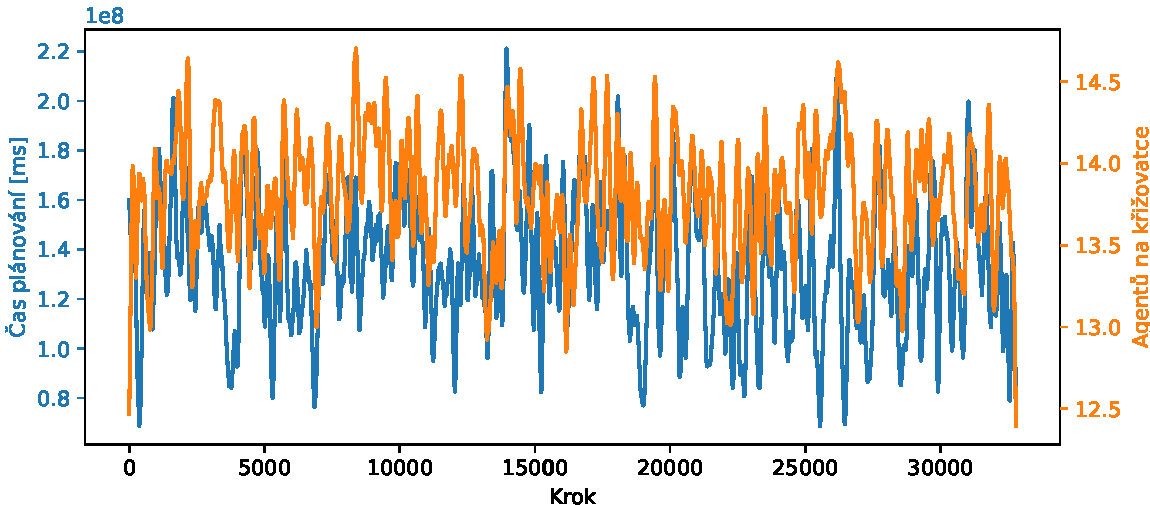
\includegraphics[width=140mm]{../img/CasVsAgentiSATRSG}
	\caption{Plánovací časy a počet naplánovaných agentů u \nameref{subsec:sat_rsg}}
	\label{fig:cas_vs_agenti_satrsg}
\end{figure}

Vytvořil jsem graf i pro \nameref{subsec:sat_ra} (Obrázek \ref{fig:cas_vs_agenti_satra}).
Tento běh byl taktéž z oktagonální křižovatky, kde algoritmus měl povolené zastavování,
\ref{str:ars_mnv} nastavené na $1$, \ref{str:ars_mpc} na $10$ a maximální počet plánovaných agentů byl $8$.

Dle mého názoru má zde mnohem větší vliv na plánování hledání modelu řešičem,
a proto je zde mnohem jasnější závislost mezi počtem agentů na křižovatce a časy plánování.
Obzvláště je zde vidět přibližně čtyřnásobná doba plánování v prvních krocích oproti průměrnému času.


\begin{figure}[h]
	\centering
	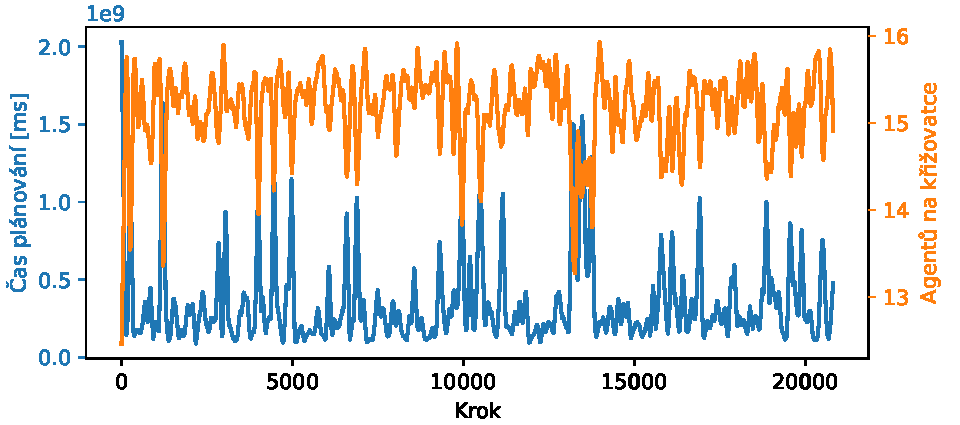
\includegraphics[width=140mm]{../img/CasVsAgentiSATRA}
	\caption{Plánovací časy a počet naplánovaných agentů u \nameref{subsec:sat_ra}}
	\label{fig:cas_vs_agenti_satra}
\end{figure}



\section{Hromadné výsledky}\label{sec:hromadne_vysledky}

%Porovnání algoritmů mezi sebou s nejlepšími parametry.
%
%Porovnání čtvercové a oktagonální křižovatky.

Nyní budu porovnávat nejlepší nastavení algoritmů mezi sebou.
Porovnání by mělo být férové, jelikož všechny algoritmy běžely s podobným nastavením parametrů.
Nejlepší nastavení většiny parametrů je zobrazeno v prvních sloupcích tabulky hned za názvem algoritmu.

Zároveň je v tabulkách obsažen algoritmus \nameref{sec:safe_lanes}.
Ten byl doposud vynechán, jelikož nemá žádné nastavitelné parametry.

\subsection{Porovnání algoritmů na malé křižovatce}\label{subsec:porovnani_algoritmu_na_male_krizovatce}

V této kapitole porovnám jednotlivé algoritmy na malých typech křižovatek.

Jediný algoritmus, který nedoběhl ani na jednom typu malé křižovatky je \nameref{subsec:cbsoid}.
Z toho usuzuji, že \ref{str:cbs} je nejvíce citlivý na přidávání agentů.


Nejprve začnu čtvercovou křižovatkou, jejíž výsledky jsou v tabulce \ref{tab:all_exp_mala_ctvercova}.
V tabulce není zapsána hodnota parametru maximálního počtu přeplánovaných agentů (\ref{par:aoid_mpa}) u~\ref{str:oid} variant.
Na této křižovatce měli \nameref{subsubsec:a_star_aoid} a \nameref{subsec:cbsoid}
největší úspěšnost s \ref{par:aoid_mpa} nastaveným na $16$ a \nameref{subsec:sat_ra} na $12$.

Nejlepší algoritmus zde vyšel \ref{str:cbs}, v těsném závěsu za ním je \ref{str:a_star_ars}.
Tyto algoritmy mají zároveň nejmenší zpoždění agentů a v průměru nejméně agentů na křižovatce.
Zároveň měli nejnižší dobu plánování po \nameref{sec:safe_lanes}.

Po těchto algoritmech měly nejmenší počet zamítnutí \ref{str:sat} algoritmy a průměrná zpoždění byla srovnatelná.
Avšak po \nameref{subsec:cbsoid} měly nejvyšší čas plánování.

\nameref{sec:safe_lanes} sice zvládlo plánovat agenty mnohem rychleji než ostatní algoritmy,
avšak zároveň má mnohem více zamítnutých agentů, než všechny algoritmy, které doběhly.

\nameref{subsubsec:a_star_aoid} měl nejvyšší průměrný počet agentů na křižovatce,
avšak zároveň měl jednoznačně nejvyšší průměrné zpoždění agentů.

Verze algoritmů plánující menší počet agentů preferovala spíše volnější pohyb pro agenty.
Naopak všechny \ref{str:oid} varianty, \nameref{subsec:sat_ra} a \ref{str:a_star_arsg} dosáhly nejlepších výsledků s nejvíce omezenými parametry.

\begin{table}[h]
%	\centering
	\begin{adjustwidth}{-0.5cm}{}
		\begin{tabular}{c c c c | r r D{.}{,}{2.2} D{.}{,}{2.2} D{.}{,}{7.2}}
			\toprule \\
			\pulrad{\B{Alg}} & \pulrad{\B{Omez}} & \pulrad{\B{\ref{str:ars_mnv}}} &
			\pulrad{\B{\ref{str:ars_mpc}}} & \pulrad{\B{Krok}}  & \pulrad{\B{Zam}} &
			\mc{\pulrad{\B{pAg}}} & \mc{\pulrad{\B{pZp}}} & \mc{\pulrad{\B{Čas}}} \\
			\midrule
			\nameref{sec:safe_lanes}        & -  & 1 & inf & 32782 & 4056   & 11.19                                & 6.89                                & \multicolumn{1}{B{.}{,}{7.2}}{16.75} \\
			\hline
			\ref{str:a_star_ars}            & s  & 2 & inf & 32775 & 76     & 13.68                                & 3.92                                & 47.77                                \\
			\ref{str:varsg}           & -  & 1 & 8   & 32779 & 568    & 14.20                                & 5.72                                & 262.71                               \\
			\nameref{subsubsec:a_star_aoid} & -  & 1 & 8   & 32786 & 1373   & \multicolumn{1}{B{.}{,}{2.2}}{18.04} & 15.10 & 5582.03                                                            \\  % 16
			\hline
			\ref{str:cbs}                   & sr & 2 & inf & 32776 & \B{70} & 13.41                                & \multicolumn{1}{B{.}{,}{2.2}}{3.66} & 194.12                               \\
			\nameref{subsec:cbsoid}         & -  & 1 & 16  & 6838  & 51759  & 12.61                                & 8.45                                & 1054679.77                           \\  % 16
			\hline
			\nameref{subsec:sat_rsg}        & s  & 2 & 24  & 32778 & 255    & 13.46                                & 3.90                                & 131515.34                            \\
			\nameref{subsec:sat_ra}         & -  & 1 & 10  & 32776 & 363    & 15.07                                & 5.44                                & 9893.10                              \\  % 12
			\bottomrule
%		\multicolumn{6}{l}{\footnotesize \textit{Pozn:}
%		\textrm{Zam} - počet zamítnutí, \textrm{pAgen} - průměrný počet agentů v jeden krok na křižovatce, \\
%		\textrm{sAgen} - směrodatná odchylka počtu agentů na křižovatce, \\
%		\textrm{Zpož} - součet spoždění přes všechny agenty, \textrm{pZpož} - průměrné zpoždění agentů
%		}  TODO
		\end{tabular}
		\caption{Porovnání algoritmů na malé čtvercové křižovatce.}\label{tab:all_exp_mala_ctvercova}
	\end{adjustwidth}
\end{table}

Na oktagonální křižovatce je chování algoritmů podobné (tabulka \ref{tab:all_exp_mala_oktagonalni}).
Avšak zde ani jeden z algoritmů přeplánovající naplánované agenty nestihl doběhnout.
Zde měli \nameref{subsubsec:a_star_aoid} a \nameref{subsec:cbsoid}
největší úspěšnost opět s \ref{par:aoid_mpa} nastaveným na $16$ a \nameref{subsec:sat_ra} na $12$.

Pořadí algoritmů, které doběhly, s ohledem na počet zamítnutých agentů se nezměnilo,
stále si nejlépe vedlo \ref{str:cbs}.

\nameref{subsubsec:a_star_aoid} opět mělo v průměru nejvíce agentů na křižovatce, ale opět nejvyšší zpoždění agentů.

\nameref{sec:safe_lanes} sice zvládlo má opět mnohem více zamítnutých agentů, než všechny algoritmy, které doběhly.
Oproti čtvercové křižovatce se plánovací časy snížily,
avšak při tak nízkých časech to může být způsobeno zatížením systému jinými procesy.

Běhové časy se u ostatních algoritmů výrazně zvýšily.
To může být způsobeno výrazným nárůstem počtu zamítnutých agentů.
Podle mého názoru je tento nárůst způsoben zmenšením celkové plochy křižovatky.
Diagonální vrcholy size umožňují více možných pozic pro agenty,
avšak tyto vrcholy jsou blízko svým sousedům, což způsobuje větší vzájemné překážení jednotlivých agentů.

Obecně bych řekl, že zde algoritmy více profitovaly z méně omezenéných parametrů,
až na \ref{str:a_star_arsg} a \nameref{subsubsec:a_star_aoid}.

\begin{table}[h]
%	\centering
	\begin{adjustwidth}{-0.5cm}{}
		\begin{tabular}{c c c c | r r D{.}{,}{2.2} D{.}{,}{2.2} D{.}{,}{7.2}}
			\toprule \\
			\pulrad{\B{Alg}} & \pulrad{\B{Omez}} & \pulrad{\B{\ref{str:ars_mnv}}} &
			\pulrad{\B{\ref{str:ars_mpc}}} & \pulrad{\B{Krok}}  & \pulrad{\B{Zam}} &
			\mc{\pulrad{\B{pAg}}} & \mc{\pulrad{\B{pZp}}} & \mc{\pulrad{\B{Čas}}} \\
			\midrule
			\nameref{sec:safe_lanes}        & -  & 1 & inf & 32785 & 13488    & 9.34                                 & 10.36                               & \multicolumn{1}{B{.}{,}{7.2}}{11.30} \\
			\hline
			\ref{str:a_star_ars}            & sr & 2 & inf & 32779 & 1338     & 14.19                                & 6.83                                & 89.03                                \\
			\ref{str:varsg}           & -  & 1 & 8   & 32785 & 6276     & 13.14                                & 9.46                                & 237.60                               \\
			\nameref{subsubsec:a_star_aoid} & -  & 1 & 8   & 16976 & 32774    & \multicolumn{1}{B{.}{,}{2.2}}{18.49} & 17.57 & 424199.33                                                          \\  % 16
			\hline
			\ref{str:cbs}                   & sr & 2 & inf & 32780 & \B{1079} & 13.91                                & \multicolumn{1}{B{.}{,}{2.2}}{6.46} & 1761.27                              \\
			\nameref{subsec:cbsoid}         & s  & 2 & inf & 2889  & 59641    & 11.99                                & 10.23                               & 2497072.06                           \\  % 16
			\hline
			\nameref{subsec:sat_rsg}        & s  & 2 & 24  & 32782 & 2868     & 13.81                                & 7.77                                & 133605.81                            \\
			\nameref{subsec:sat_ra}         & s  & 1 & 10  & 20821 & 25521    & 15.16                                & 8.57                                & 345728.00                            \\  %  8
			\bottomrule
%		\multicolumn{6}{l}{\footnotesize \textit{Pozn:}
%		\textrm{Zam} - počet zamítnutí, \textrm{pAgen} - průměrný počet agentů v jeden krok na křižovatce, \\
%		\textrm{sAgen} - směrodatná odchylka počtu agentů na křižovatce, \\
%		\textrm{Zpož} - součet spoždění přes všechny agenty, \textrm{pZpož} - průměrné zpoždění agentů
%		}  TODO
		\end{tabular}
		\caption{Porovnání algoritmů na malé oktagonální křižovatce.}\label{tab:all_exp_mala_oktagonalni}
	\end{adjustwidth}
\end{table}

Jelikož tato křižovatka obsahuje téměř dvakrát více vrcholů, než oktagonální, $48$ oproti $28$, čekal jsem,
že běhové časy algoritmů budou značně horší než na oktagonální křižovatce.
Avšak první pohled na tabulku \ref{tab:all_exp_mala_hexagonalni}, kde jsou zapsaná výsledky, napovídá opaku.

Jediný algoritmus, který nedoběhl, je opět \nameref{subsec:cbsoid}.
Avšak pokud srovnám časy plánování mezi předchozí křižovatkou a touto, jediné algoritmy, které si polepšily,
jsou \nameref{subsubsec:a_star_aoid} a \ref{str:sat} algoritmy.
Podle mého názoru je tomuto jevu značně pomohlo snížení počtu přeplánovaných agentů.
Ten totiž měl u \nameref{subsubsec:a_star_aoid} hodnotu $12$,
u \nameref{subsec:cbsoid} $24$ a u \nameref{subsec:sat_ra} $8$.

Zároveň u \nameref{subsec:sat_rsg} stoupla průměrná zaplňenost křižovatky z přibližně $49,32\%$ na $54,56\%$.
Jak jsem popsal u v kapitole s výsledky pro \ref{str:sat} (Kapitola \ref{subsubsec:sat_zavislost_casu_a_agentu}),
\ref{str:sat} algoritmy mají menší plánovací čas s více zaplněnou křižovatkou.
Avšak nemyslím si, že je toto hlavní důvod zrychlení, jelikož i když je zaplněnost křižovatky vyšší,
celkový počet vrcholů je značně vyšší, čili průměrný počet volných vrcholů se zvýšil.
Osobně si myslím, že je rozdíl v časech způsobený nižším nastavením parametru \ref{par:ars_mpc}
u~\nameref{subsec:sat_rsg}, a nižším počtem přeplánovaných agentů u~\nameref{subsec:sat_ra}.

Překvapivě na této křižovatce má nejméně zamítnutých agentů a nejmenší zpoždění zmiňovaný \nameref{subsec:sat_ra}.
Mimo to je pořadí algoritmů z pohledu na počet zamítnutých agentů totožné s pořadím na čtvercové křižovatce.
Druhý nejlepší je \ref{cbs}, následuje \ref{str:a_star_ars}, \nameref{subsec:sat_rsg}, \ref{str:a_star_arsg}
a \nameref{subsubsec:a_star_aoid}.
Nejhorším úspěšně doběhnutým algoritmem je opět \nameref{sec:safe_lanes}.

\begin{table}[h]
%	\centering
	\begin{adjustwidth}{-0.5cm}{}
		\begin{tabular}{c c c c | r r D{.}{,}{2.2} D{.}{,}{2.2} D{.}{,}{7.2}}
			\toprule \\
			\pulrad{\B{Alg}} & \pulrad{\B{Omez}} & \pulrad{\B{\ref{str:ars_mnv}}} &
			\pulrad{\B{\ref{str:ars_mpc}}} & \pulrad{\B{Krok}}  & \pulrad{\B{Zam}} &
			\mc{\pulrad{\B{pAg}}} & \mc{\pulrad{\B{pZp}}} & \mc{\pulrad{\B{Čas}}} \\
			\midrule
			\nameref{sec:safe_lanes}        & -  & 1 & inf & 32796 & 32273    & 14.15                                & 18.18                               & \multicolumn{1}{B{.}{,}{7.2}}{87.44} \\
			\hline
			\ref{str:a_star_ars}            & s  & 2 & inf & 32790 & 3021     & 26.54                                & 11.08                               & 734.08                               \\
			\ref{str:varsg}           & -  & 1 & 16  & 32792 & 5872     & 25.94                                & 13.15                               & 1195.23                              \\
			\nameref{subsubsec:a_star_aoid} & s  & 2 & 16  & 32800 & 9472     & \multicolumn{1}{B{.}{,}{2.2}}{32.67} & 21.81                               & 10276.77                             \\  %  12
			\hline
			\ref{str:cbs}                   & sr & 2 & inf & 32790 & 2698     & 25.74                                & 10.80                               & 3128.19                              \\
			\nameref{subsec:cbsoid}         & s  & 2 & inf & 1704  & 93403    & 22.16                                & 21.18                               & 4255409.05                           \\  % 24
			\hline
			\nameref{subsec:sat_rsg}        & -  & 1 & 16  & 32787 & 4403     & 26.19                                & 12.08                               & 78214.86                             \\
			\nameref{subsec:sat_ra}         & -  & 1 & 10  & 32788 & \B{1905} & 26.06                                & \multicolumn{1}{B{.}{,}{2.2}}{8.85}  & 34920.59                            \\  %  8
			\bottomrule
%		\multicolumn{6}{l}{\footnotesize \textit{Pozn:}
%		\textrm{Zam} - počet zamítnutí, \textrm{pAgen} - průměrný počet agentů v jeden krok na křižovatce, \\
%		\textrm{sAgen} - směrodatná odchylka počtu agentů na křižovatce, \\
%		\textrm{Zpož} - součet spoždění přes všechny agenty, \textrm{pZpož} - průměrné zpoždění agentů
%		}  TODO
		\end{tabular}
		\caption{Porovnání algoritmů na malé hexagonální křižovatce.}\label{tab:all_exp_mala_hexagonalni}
	\end{adjustwidth}
\end{table}

Z uvedených výsledků usuzuji, že na malých křižovatkách se mnohem více vyplatí jednodušší, více omezené algoritmy.
Vypadá to, že pokud algoritmus přeplánovává agenty, vyplatí se měnit pouze malé množství agentů.
\nameref{sec:safe_lanes} plánuje agenty hodně rychle, avšak za cenu vysokého počtu zamítnutých agentů.

\subsection{Porovnání algoritmů na velké křižovatce bez výjezdů}
\label{subsec:porovnani_algoritmu_na_velke_krizovatce_bez_vyjezdu}

V této sekci jsou porovnány pouze algoritmy, které zvládly alespoň částečně něco spočítat.
\ref{str:sat} algoritmy nezvládly výpočet ani na jediném typu křižovatky.
\nameref{subsubsec:a_star_aoid} úspěšně běžel jenom na čtvercové křižovatce, na zbylých padal kvůli paměťové náročnosti.
\nameref{subsec:cbsoid} byl kvůli času neúspěšný na hexagonálním typu.

Výsledky pro čtvercovou křižovatku (\ref{tab:all_exp_velka_ctvercova_bez_vyjezdu}) obsahují určité překvapivé hodnoty.
Zde algoritmy \nameref{subsubsec:a_star_aoid} i \nameref{subsec:cbsoid} plánovaly nejvýše $32$ agentů každý krok.

\nameref{subsubsec:a_star_aoid} opět dosáhl největšího zaplnění křižovatky.
Avšak tentokrát měl i nejnižší počet zamítnutých agentů.

Proto mě překvapuje, že \ref{str:a_star_arsg} měl druhý nejvyšší počet zamítnutí hned po \nameref{sec:safe_lanes}.
Nepočítám tedy \nameref{subsec:cbsoid}, který nespočítal skoro žádné kroky.

Jediný důvod, proč toto nastalo, je podle mě vysoké množství spojování skupin u \ref{str:a_star_arsg},
které vede k dlouhé době plánování.
To způsobí, že algoritmus přejde do zjednodušeného počítání, ve kterém zamítá agenty místo snahy o přeplánování.
Ačkoliv \nameref{subsubsec:a_star_aoid} má mnohem vyšší dobu běhu, je možné, že se algoritmus \uv{zasekne}
na pár krocích, ale ve zbytku kroků je rychlejší a úspěšnější.

\ref{str:cbs} dosáhl menšího počtu zamítnutí než \ref{str:a_star_ars}, avšak za cenu vyššího průměrného zpoždění.

Řekl bych, že na této křižovatce algoritmy preferovaly menší omezení parametrů.
Algoritmy, u~kterých nezvítězily nejméně omezené varianty, byly většinou s vysokým časem běhu.

\begin{table}[h]
%	\centering
	\begin{adjustwidth}{-1cm}{}
	\begin{tabular}{c c c c | r r D{.}{,}{3.2} D{.}{,}{2.2} D{.}{,}{7.2}}
		\toprule \\
		\pulrad{\B{Alg}} & \pulrad{\B{Omez}} & \pulrad{\B{\ref{par:ars_mnv}}} &
		\pulrad{\B{\ref{par:ars_mpc}}} & \pulrad{\B{Krok}}  & \pulrad{\B{Zam}} &
		\mc{\pulrad{\B{pAg}}} & \mc{\pulrad{\B{pZp}}} & \mc{\pulrad{\B{Čas}}} \\
		\midrule
		\nameref{sec:safe_lanes}        & -  & 1 & inf & 32849 & 75983     & 86.91                                 & 44.18                                & \multicolumn{1}{B{.}{,}{7.2}}{1449.67} \\
		\hline
		\ref{str:a_star_ars}            & sr & 2 & inf & 32847 & 16461     & 138.36                                & \multicolumn{1}{B{.}{,}{2.2}}{26.71} & 11011.56   \\
		\ref{str:a_star_arsg}           & sr & 2 & inf & 32847 & 22451     & 145.58                                & 43.62                                & 21190.45                               \\
		\nameref{subsubsec:a_star_aoid} & -  & 1 & 32  & 32840 & \B{11285} & \multicolumn{1}{B{.}{,}{3.2}}{159.15} & 35.46 & 204258.46  \\  % 32
		\hline
		\ref{str:cbs}                   & s  & 2 & inf & 32848 & 13193     & 137.94                                & 31.45                                & 69699.31                               \\
		\nameref{subsec:cbsoid}         & -  & 1 & 32  & 965   & 255430    & 121.15                                & 45.84                                & 7631472.87                             \\  % 32
		\bottomrule
%		\multicolumn{6}{l}{\footnotesize \textit{Pozn:}
%		\textrm{Zam} - počet zamítnutí, \textrm{pAgen} - průměrný počet agentů v jeden krok na křižovatce, \\
%		\textrm{sAgen} - směrodatná odchylka počtu agentů na křižovatce, \\
%		\textrm{Zpož} - součet spoždění přes všechny agenty, \textrm{pZpož} - průměrné zpoždění agentů
%		}  TODO
	\end{tabular}
	\caption{Porovnání algoritmů na velké čtvercové křižovatce bez výjezdů.}\label{tab:all_exp_velka_ctvercova_bez_vyjezdu}
	\end{adjustwidth}
\end{table}


Pro oktagonální křižovatku jsou výsledky v tabulce \ref{tab:all_exp_velka_oktagonalni_bez_vyjezdu}.
Zde jediné algoritmy, které úspěšně dopočítaly všechny kroky, byly
\nameref{sec:safe_lanes}, \ref{str:a_star_ars} a \ref{str:a_star_arsg}, proto se zaměřím převážně na ně.

\ref{str:a_star_ars} zde dosáhl nejnižšího počtu zamítnutých agentů a zaplněnosti křižovatky.

Jelikož \ref{str:a_star_arsg} měla průměrně méně agentů na křižovatce než \ref{str:a_star_ars}, myslím si,
že \ref{str:a_star_arsg} často přešel do zjednodušeného režimu, čož asi způsobilo takové velké množství zamítnutí.
Díky tomu ale nejspíše dosáhl nejnižšího průměrného zpoždění agentů, jelikož křižovatka byla v průměru volnější.

Překvapením jsou plánovací časy algoritmů.
\ref{str:a_star_arsg} dosáhla výrazně rychlejšího plánování, než \ref{str:a_star_ars}.
\ref{str:a_star_ars} měl méně omezené cesty agentů, což mohlo způsobit tento velký rozdíl.
Množství možných cest pro agenta je díky tomu mnohem vyšší, což vede na mnohem více výpočtů,
než algoritmus zamítne vjezd agentovi.

\begin{table}[h]
%	\centering
	\begin{adjustwidth}{-1cm}{}
	\begin{tabular}{c c c c | r r D{.}{,}{3.2} D{.}{,}{2.2} D{.}{,}{8.2}}
		\toprule \\
		\pulrad{\B{Alg}} & \pulrad{\B{Omez}} & \pulrad{\B{\ref{str:ars_mnv}}} &
		\pulrad{\B{\ref{str:ars_mpc}}} & \pulrad{\B{Krok}}  & \pulrad{\B{Zam}} &
		\mc{\pulrad{\B{pAg}}} & \mc{\pulrad{\B{pZp}}} & \mc{\pulrad{\B{Čas}}} \\
		\midrule
		\nameref{sec:safe_lanes} & -  & 1 & inf & 32846 & 107830   & 71.98                                 & 58.92                                & \multicolumn{1}{B{.}{,}{8.2}}{1914.34} \\
		\hline
		\ref{str:a_star_ars}     & s  & 2 & inf & 32837 & \B{6046} & \multicolumn{1}{B{.}{,}{3.2}}{157.83} & 25.65 & 117705.81   \\
		\ref{str:varsg}    & -  & 1 & 32  & 32840 & 12990    & 142.63                                & \multicolumn{1}{B{.}{,}{2.2}}{19.84} & 62133.51    \\
		\hline
		\ref{str:cbs}            & sr & 2 & inf & 10221 & 184171   & 146.21                                & 26.42                                & 705203.89                              \\
		\nameref{subsec:cbsoid}  & sr & 2 & inf & 638   & 257862   & 118.79                                & 47.18                                & 11697421.69                            \\  % 32
		\bottomrule
%		\multicolumn{6}{l}{\footnotesize \textit{Pozn:}
%		\textrm{Zam} - počet zamítnutí, \textrm{pAgen} - průměrný počet agentů v jeden krok na křižovatce, \\
%		\textrm{sAgen} - směrodatná odchylka počtu agentů na křižovatce, \\
%		\textrm{Zpož} - součet spoždění přes všechny agenty, \textrm{pZpož} - průměrné zpoždění agentů
%		}  TODO
	\end{tabular}
	\caption{Porovnání algoritmů na velké oktagonální křižovatce bez výjezdů.}\label{tab:all_exp_velka_oktagonalni_bez_vyjezdu}
	\end{adjustwidth}
\end{table}


Hexagonální křižovatka obsahuje mnohem více vrcholů, než oktagonální.
Proto není divu,
že tabulka s výsledky pro tuto křižovatku obsahuje ještě méně záznamů (\ref{tab:all_exp_velka_hexagonalni_bez_vyjezdu}).

Tabulka neobsahuje moc zajímavých hodnot, jelikož jediné algoritmy, které úspěšně dopočítaly všechny kroky až do konce,
jsou \nameref{sec:safe_lanes} a \ref{str:a_star_ars}.
\ref{str:a_star_ars} má vyšší výpočetní dobu, avšak mnohem nižší počet zamítnutí.

Překvapilo mě jenom, že i když \ref{str:a_star_ars} mělo méně omezené agenty než na oktagonální křižovatce,
časy plánování zůstaly přibližně stejné.
Na oktagonální křižovatce tento algoritmus zamítl přibližně $2,3\%$ agentů, avšak na hexagonální celých $13,56\%$.
Avšak zaplnění křižovatky byl na oktagonální křižovatce $31.07\%$, zatímco na hexagonální $37.4\%$.
Zároveň na hexagonální křižovatce bylo mnohem vyšší průměrné zpoždění agentů.
Proto si myslím, že na hexagonální křižovatce si agenti mnohem více překážejí.
Myslím si, že to způsobuje snazší a rychlejší zjištění, že neexistuje pro daného agenta žádná cesta.
Podle mého je toto hlavní důvod, proč není výrazné zvýšení plánovacího času.

\begin{table}[h]
%	\centering
	\begin{adjustwidth}{-1cm}{}
	\begin{tabular}{c c c c | r r D{.}{,}{3.2} D{.}{,}{2.2} D{.}{,}{7.2}}
		\toprule \\
		\pulrad{\B{Alg}} & \pulrad{\B{Omez}} & \pulrad{\B{\ref{str:ars_mnv}}} &
		\pulrad{\B{\ref{str:ars_mpc}}} & \pulrad{\B{Krok}}  & \pulrad{\B{Zam}} &
		\mc{\pulrad{\B{pAg}}} & \mc{\pulrad{\B{pZp}}} & \mc{\pulrad{\B{Čas}}} \\
		\midrule
		\nameref{sec:safe_lanes} & -  & 1 & inf & 32894 & 212628    & 109.63                                & 92.37                                & \multicolumn{1}{B{.}{,}{7.2}}{4221.17} \\
		\hline
		\ref{str:a_star_ars}     & sr & 2 & inf & 32893 & \B{35567} & 287.20                                & \multicolumn{1}{B{.}{,}{2.2}}{48.34} & 128608.45  \\
		\ref{str:varsg}    & s  & 2 & inf & 20359 & 198896    & \multicolumn{1}{B{.}{,}{3.2}}{299.14} & 88.14 & 353255.32  \\
		\hline
		\ref{str:cbs}            & s  & 2 & inf & 4011  & 347852    & 292.50                                & 59.07                                & 1810300.99                             \\
		\bottomrule
%		\multicolumn{6}{l}{\footnotesize \textit{Pozn:}
%		\textrm{Zam} - počet zamítnutí, \textrm{pAgen} - průměrný počet agentů v jeden krok na křižovatce, \\
%		\textrm{sAgen} - směrodatná odchylka počtu agentů na křižovatce, \\
%		\textrm{Zpož} - součet spoždění přes všechny agenty, \textrm{pZpož} - průměrné zpoždění agentů
%		}  TODO
	\end{tabular}
	\caption{Porovnání algoritmů na velké hexagonální křižovatce bez výjezdů.}\label{tab:all_exp_velka_hexagonalni_bez_vyjezdu}
	\end{adjustwidth}
\end{table}


\subsection{Porovnání algoritmů na velké křižovatce s výjezdy}
\label{subsec:porovnani_algoritmu_na_velke_krizovatce_s_vyjezdy}

Na velkých křižovatkách s výjezdy zvládlo úspěšně spočítat nemalé množství kroků ještě méně algoritmů.
Omezení z více výjezdů pouze na jeden zesložití hledání cesty, což povede k delším cestám.
Čím déle jsou agenti na křižovatce, tím více překáží ostatním agentům.
Toto by se obzvláště mělo projevit u \ref{str:rsg}, \ref{subsec:sat_ra} a \ref{str:oid} strategií,
protože musí nějakým způsobem hledat a řešit vzájemné kolize agentů.
Oba tyto jevy by zde měly být těžší už jen kvůli delším cestám.

Výsledky pro čtvercovou křižovatku jsou v tabulce \ref{tab:all_exp_velka_ctvercova_s_vyjezdy}.
Na této křižovatce byl \nameref{subsec:cbsoid} nejlepší s $24$ nejvýše plánovanými agenty.
Avšak ani tak nezvládl tento algoritmus naplánovat příliš mnoho kroků.

\ref{str:cbs} zde dosáhl nejmenšího počtu zamítnutí a druhého nejmenšího průměrného zpoždění.
\ref{str:a_star_ars} bylo mírně horší s ohledem na zamítnuté agenty, ale zato měl mnohem menší plánovací čas.
\ref{str:a_star_arsg} byl také poměrně rychlý, avšak zamítl mnohem více agentů.

Pokud porovnám výsledky s běhy na~čtvercové křižovatce bez výjezdů,
všechny algoritmy si zhoršily počet zamítnutých agentů i průměrné zpoždění.
Zároveň se u všech algoritmů až na~\nameref{sec:safe_lanes} prodloužily plánovací časy.
Těmto algoritmům se i zvýšilo průměrné zaplnění křižovatky.

Zkrácení času plánování u \ref{sec:safe_lanes} není překvapivé, jelikož algoritmus zkouší méně možných cest.

Pokud algoritmus doběhl, dosáhl nejlepších výsledků s nejméně omezenými parametry.

\begin{table}[h]
%	\centering
	\begin{adjustwidth}{-1cm}{}
		\begin{tabular}{c c c c | r r D{.}{,}{3.2} D{.}{,}{2.2} D{.}{,}{7.2}}
			\toprule \\
			\pulrad{\B{Alg}} & \pulrad{\B{Omez}} & \pulrad{\B{\ref{par:ars_mnv}}} &
			\pulrad{\B{\ref{par:ars_mpc}}} & \pulrad{\B{Krok}}  & \pulrad{\B{Zam}} &
			\mc{\pulrad{\B{pAg}}} & \mc{\pulrad{\B{pZp}}} & \mc{\pulrad{\B{Čas}}} \\
			\midrule
			\nameref{sec:safe_lanes} & -  & 1 & inf & 32850 & 111987    & 77.02                                 & 60.70                                & \multicolumn{1}{B{.}{,}{7.2}}{1244.95} \\
			\hline
			\ref{str:a_star_ars}     & sr & 2 & inf & 32846 & 26667     & 155.96                                & \multicolumn{1}{B{.}{,}{2.2}}{35.99} & 14428.00   \\
			\ref{str:a_star_arsg}    & sr & 2 & inf & 32855 & 40413     & \multicolumn{1}{B{.}{,}{3.2}}{159.59} & 52.69 & 49668.90   \\
			\hline
			\ref{str:cbs}            & sr & 2 & inf & 32846 & \B{23949} & 155.63                                & 36.41                                & 160418.65                              \\
			\nameref{subsec:cbsoid}  & -  & 1 & 64  & 957   & 255758    & 136.49                                & 52.40                                & 7736125.71                             \\  % 24
			\bottomrule
%		\multicolumn{6}{l}{\footnotesize \textit{Pozn:}
%		\textrm{Zam} - počet zamítnutí, \textrm{pAgen} - průměrný počet agentů v jeden krok na křižovatce, \\
%		\textrm{sAgen} - směrodatná odchylka počtu agentů na křižovatce, \\
%		\textrm{Zpož} - součet spoždění přes všechny agenty, \textrm{pZpož} - průměrné zpoždění agentů
%		}  TODO
		\end{tabular}
		\caption{Porovnání algoritmů na velké čtvercové křižovatce s výjezdy.}\label{tab:all_exp_velka_ctvercova_s_vyjezdy}
	\end{adjustwidth}
\end{table}


Na oktagonální křižovatce doběhly pro všechny kroky pouze
\nameref{sec:safe_lanes}, \ref{str:a_star_ars} a \ref{str:a_star_arsg}.

Nejméně zamítnutí a nejmenší zpoždění měl \ref{str:a_star_ars}.
Myslím si, že i zde nastal dříve popsaný problém u \ref{str:a_star_arsg} s tvorbou velkých skupin.

Oproti běhům, kde agenti neměli specifikovaný výjezd,
se u všech úspěšných algoritmů opět zvýšil počet zamítnutých agentů a průměrné zpoždění.
Zároveň u \nameref{sec:a_star} variant se zvýšil průměrný počet agentů na křižovatce.
U \nameref{sec:safe_lanes} a \ref{str:a_star_ars} plánovací časy značně klesly,
avšak u \ref{str:a_star_arsg} výrazně stouply.

To napovídá možnosti, že \ref{str:a_star_ars} pro agenty existuje mnohem méně možných cest.
Avšak jelikož je celkový počet zamítnutých agentů vyšší, domnívám se,
že\ref{str:a_star_arsg} shlukuje častěji agenty do skupin, což vede k delšímu plánování.

Algoritmy zde opět měly nejlepší výsledky, pokud běžely s nejmenším omezením.

\begin{table}[h]
%	\centering
	\begin{adjustwidth}{-1cm}{}
		\begin{tabular}{c c c c | r r D{.}{,}{3.2} D{.}{,}{2.2} D{.}{,}{7.2}}
			\toprule \\
			\pulrad{\B{Alg}} & \pulrad{\B{Omez}} & \pulrad{\B{\ref{par:ars_mnv}}} &
			\pulrad{\B{\ref{par:ars_mpc}}} & \pulrad{\B{Krok}}  & \pulrad{\B{Zam}} &
			\mc{\pulrad{\B{pAg}}} & \mc{\pulrad{\B{pZp}}} & \mc{\pulrad{\B{Čas}}} \\
			\midrule
			\nameref{sec:safe_lanes} & -  & 1 & inf & 32849 & 138867    & 61.62                                 & 60.30                                & \multicolumn{1}{B{.}{,}{7.2}}{937.51} \\
			\hline
			\ref{str:a_star_ars}     & sr & 2 & inf & 32844 & \B{24714} & \multicolumn{1}{B{.}{,}{3.2}}{164.83} & \multicolumn{1}{B{.}{,}{2.2}}{34.25} & 72598.43   \\
			\ref{str:a_star_arsg}    & sr & 2 & inf & 32855 & 36807     & 163.73                                & 52.16                                & 145805.57                             \\
			\hline
			\ref{str:cbs}            & s  & 2 & inf & 6774  & 212658    & 159.57                                & 43.74                                & 1065891.74                            \\

			\bottomrule
%		\multicolumn{6}{l}{\footnotesize \textit{Pozn:}
%		\textrm{Zam} - počet zamítnutí, \textrm{pAgen} - průměrný počet agentů v jeden krok na křižovatce, \\
%		\textrm{sAgen} - směrodatná odchylka počtu agentů na křižovatce, \\
%		\textrm{Zpož} - součet spoždění přes všechny agenty, \textrm{pZpož} - průměrné zpoždění agentů
%		}  TODO
		\end{tabular}
		\caption{Porovnání algoritmů na velké oktagonální křižovatce s výjezdy.}\label{tab:all_exp_velka_oktagonalni_s_vyjezdy}
	\end{adjustwidth}
\end{table}


V tabulce \ref{tab:all_exp_velka_hexagonalni_s_vyjezdy} jsou vidět výsledky pro hexagonální křižovatku.
Zde úspěšně spočetly všechny kroky pouze \nameref{sec:safe_lanes} a \ref{str:a_star_ars}.

Zde opět \ref{str:a_star_ars} nejlépě běžel s nejmenším omezením.
Oproti variantě bez výjezdů měl algoritmus vyšší zaplněnost křižovatky, průměrné zpoždění agentů i plánovací čas.
Avšak počet zamítnutých agentů se mírně snížil.

Důvod tohoto snížení neznám, avšak vzhledem k chování na předešlých typech si myslím,
že je to dáno vzhledem křižovatky.
Na hexagonální křižovatce nemohou jezdit agenti rovně do protějšího výjezdu a proto musí jet netriviální cestou.
Pokud specifikujeme výjezd, nejspíše to má minimální vliv na chování agenta.

Tomu napovídá i změna v průměrném zpoždění a obsazenosti křižovatky.
Na této křižovatce je tato změna mnohem menší než na čtvercové a oktagonální.

\nameref{sec:safe_lanes} se chová pořád stejně, plánovací čas se snížil a
počet zamítnutých agentů i průměrné zpoždění se zvýšilo.

\begin{table}[h]
%	\centering
	\begin{adjustwidth}{-1cm}{}
		\begin{tabular}{c c c c | r r D{.}{,}{3.2} D{.}{,}{2.2} D{.}{,}{7.2}}
			\toprule \\
			\pulrad{\B{Alg}} & \pulrad{\B{Omez}} & \pulrad{\B{\ref{str:ars_mnv}}} &
			\pulrad{\B{\ref{str:ars_mpc}}} & \pulrad{\B{Krok}}  & \pulrad{\B{Zam}} &
			\mc{\pulrad{\B{pAg}}} & \mc{\pulrad{\B{pZp}}} & \mc{\pulrad{\B{Čas}}} \\
			\midrule
			\nameref{sec:safe_lanes} & -  & 1 & inf & 32893 & 234142    & 99.14                                 & 92.83                                & \multicolumn{1}{B{.}{,}{7.2}}{2399.98} \\
			\hline
			\ref{str:a_star_ars}     & sr & 2 & inf & 32894 & \B{35385} & 316.87                                & \multicolumn{1}{B{.}{,}{2.2}}{53.93} & 211489.82  \\
			\ref{str:varsg}    & s  & 2 & inf & 15656 & 240581    & \multicolumn{1}{B{.}{,}{3.2}}{331.02} & 93.02 & 459814.95  \\
			\hline
			\ref{str:cbs}            & s  & 2 & inf & 4580  & 341093    & 312.39                                & 67.51                                & 1583005.68                             \\
			\bottomrule
%		\multicolumn{6}{l}{\footnotesize \textit{Pozn:}
%		\textrm{Zam} - počet zamítnutí, \textrm{pAgen} - průměrný počet agentů v jeden krok na křižovatce, \\
%		\textrm{sAgen} - směrodatná odchylka počtu agentů na křižovatce, \\
%		\textrm{Zpož} - součet spoždění přes všechny agenty, \textrm{pZpož} - průměrné zpoždění agentů
%		}  TODO
		\end{tabular}
		\caption{Porovnání algoritmů na velké hexagonální křižovatce s výjezdy.}\label{tab:all_exp_velka_hexagonalni_s_vyjezdy}
	\end{adjustwidth}
\end{table}



%\section{Neoptimální agenti}\label{sec:neoptimalni_agenti}

%Vzájemné porovnání algoritmů při datech, kdy křižovatka má nepřesná data o agentech.
